% A tool for Formal Verification of Probabilistic Spiking Neural Networks
% via Weight-Discretized Quotient Abstractions
%
% ICANN 2026 — CAMERA-READY (Springer LNCS). Max 12 pages INCLUDING references.
% Ported from the accepted Typst source (camera_ready.typ, review=false pass).
%
% Build:  pdflatex main && bibtex main && pdflatex main && pdflatex main
%
\documentclass[runningheads]{llncs}

\usepackage[T1]{fontenc}
\usepackage[utf8]{inputenc}
\usepackage{graphicx}
\usepackage{amsmath,amssymb,amsfonts}
\usepackage[hidelinks]{hyperref}
\urlstyle{rm}  % URLs in roman (matches body), consistent with raw-text DOIs from splncs04

\begin{document}

\title{A tool for Formal Verification of Probabilistic Spiking Neural Networks
  via Weight-Discretized Quotient Abstractions}
\titlerunning{Formal Verification of SNNs via Weight-Discretized Quotient Abstractions}

\author{Nikan Zandian Jazi \and Elisabetta De Maria \and Christopher Leturc}
\authorrunning{N. Zandian Jazi, E. De Maria, C. Leturc}

\institute{Université Côte d'Azur, CNRS, I3S, France\\
  \email{\{zandian,edemaria,leturc\}@i3s.unice.fr}}

\maketitle

\begin{abstract}
Spiking Neural Networks (SNNs) model biological neural dynamics more
faithfully than classical artificial networks, but their stochastic,
event-driven computation demands probabilistic models for which
deterministic abstractions are inadequate. Formal verification via
probabilistic model checking then faces a fundamental barrier: the
\emph{state space explosion problem}, where the transition system grows
exponentially with the number of neurons. General-purpose quotient model
abstractions can in principle mitigate this growth by partitioning membrane
potentials into equivalence classes, but a naïve application to SNNs discards
synaptic weight information, limiting the properties that can be verified.
This paper introduces a \emph{weight-discretized quotient model abstraction}
that maps continuous synaptic weights to a compact integer range while
preserving the relative contribution of each synapse, and presents CogSpike, a
unified workbench that integrates probabilistic SNN design, simulation, and
PRISM-based formal verification within a single tool chain. The discretization
is accompanied by formal correctness guarantees: a Threshold Preservation
theorem ensures that firing configurations with sufficient margin are
preserved, and an Asymptotic Silence theorem guarantees that spurious firing
cannot persist. A case study on contralateral inhibition demonstrates the full
design--simulate--verify workflow and confirms that the discretized model
preserves Winner-Takes-All dynamics with a $9.3\times$ state space reduction.

\keywords{Spiking Neural Networks \and Formal Verification \and Model Checking
  \and PRISM \and Quotient Abstraction \and Weight Discretization}
\end{abstract}


% ═══════════════════════════════════════════════════════════════════════════
\section{Introduction}\label{sec:intro}

Spiking Neural Networks (SNNs), the third generation of artificial neural
networks~\cite{maass1997networks}, are modelled as directed graphs whose nodes
represent neurons and whose edges represent synaptic connections that can be
either \emph{excitatory} (positive weight) or \emph{inhibitory} (negative
weight). Unlike rate-coded deep networks, SNNs communicate via discrete,
asynchronous spikes whose precise timing encodes information alongside aggregate
firing rates, making them a natural candidate for studying how real neural
circuits process and transmit information. Among SNN neuron models, the Leaky
Integrate-and-Fire (LIF) formulation provides analytical tractability, while
biophysically detailed models such as Hodgkin--Huxley~\cite{hodgkin1952quantitative}
and computationally efficient alternatives such as Izhikevich
neurons~\cite{izhikevich2003simple} reproduce a wider repertoire of biological
firing patterns at higher computational cost.

Understanding how the brain computes requires studying the \emph{temporal
dynamics} of neural circuits---how spikes propagate, interact, and give rise to
emergent behaviours in small but functionally relevant topologies such as
chains, convergent motifs, and recurrent loops. Modelling these dynamics demands
a delicate balance: biological neurons are inherently stochastic---ion-channel
noise, unreliable vesicle release, and variable axonal delays inject randomness
at every stage~\cite{hodgkin1952quantitative,nguyen2021review}, so probabilistic
models are necessary.

One promising avenue encodes the network as a Discrete-Time Markov Chain (DTMC):
probabilistic model checking can then determine whether the DTMC satisfies the
behavioural properties expected by neuroscientists, such as tonic spiking under
sustained input or silence without stimulation~\cite{naco20}. However, this
approach faces a fundamental barrier: the \emph{state space explosion problem},
where the DTMC state space grows exponentially with network size, rendering
verification intractable beyond a handful of neurons.

This paper addresses that challenge. We propose CogSpike, a unified tool for
probabilistic spiking neural networks that integrates three tightly coupled
capabilities within a single framework: (i)~\emph{simulation} of probabilistic
LIF-based SNN dynamics, (ii)~\emph{formal modelling} of the same networks as
DTMCs for the PRISM model checker~\cite{PRISM2011} (a tool that computes the
probability with which a temporal-logic property holds over a DTMC, up to
floating-point precision), and (iii)~\emph{automated model checking} of
behavioural properties expressed in Probabilistic Computation Tree Logic
(PCTL)~\cite{hansson1994logic}. The underlying neuron model employs a
weight-discretized quotient abstraction that overcomes the limitations of naïve
quotient models~\cite{BaierKatoen2008}, which discard synaptic weight
information when partitioning states into equivalence classes.

Concretely, the contributions are threefold:
(1)~a \emph{weight discretization scheme} that maps continuous synaptic weights
to a finite discrete range while preserving threshold feasibility and relative
synaptic contributions;
(2)~a \emph{Threshold Preservation} theorem ensuring that firing patterns with
sufficient margin are preserved by the discretization, and an \emph{Asymptotic
Silence} theorem guaranteeing that the discretized model cannot sustain spurious
firing; and
(3)~\textbf{CogSpike}\footnote{All code and experiments are available at
\url{https://github.com/QuietRocket/CogSpike}.}, a unified workbench integrating
SNN design, simulation, and formal verification, whose code generator produces a
PRISM representation isomorphic to the simulation engine, enabling automated
formal modelling and model checking. The complete formal proofs, additional
derivations, and an empirical scaling study across seven canonical topologies
are provided in the extended version of this paper~\cite{cogspikeExtended}.
The remainder surveys related work (Section~\ref{sec:related}) and background
(Section~\ref{sec:prelim}), presents the weight-discretized abstraction
(Section~\ref{sec:weight-disc}) and the CogSpike workbench
(Section~\ref{sec:cogspike}), and reports a contralateral-inhibition case study
(Section~\ref{sec:casestudy}).


% ═══════════════════════════════════════════════════════════════════════════
\section{Related Work}\label{sec:related}

Biological neurons exhibit significant trial-to-trial variability even under
identical stimulation~\cite{gerstner2002spiking}. Classical approaches capture
this stochasticity through three mechanisms: \emph{escape noise}, which
introduces a probabilistic firing threshold; \emph{diffusive noise}, modelling
stochastic spike arrivals via synaptic bombardment; and \emph{slow noise}, which
adds fluctuations to neuronal parameters~\cite{gerstner2002spiking}. These
formulations underpin large-scale analyses of noisy integrate-and-fire
networks~\cite{brunel1999fast}, but they operate in continuous state spaces and
do not yield discrete-state models amenable to exhaustive formal verification.
Among existing simulators, Brian~2~\cite{stimberg2019brian2} supports stochastic
firing thresholds via escape noise (SDE integration), while
Nengo~\cite{bekolay2014nengo}, NEST~\cite{gewaltig2007nest}, and
BindsNET~\cite{hazan2018bindsnet} are limited to noise injection at the input
level. Crucially, none of these platforms support probabilistic model checking.

Our model takes a different route: rather than adding continuous noise to a
differential equation, we discretize the membrane potential into threshold
levels and assign each level an explicit firing probability, yielding a
finite-state probabilistic model that maps directly onto a DTMC. This enables
exhaustive formal verification via model checking, a capability that is
fundamentally unavailable with continuous-noise formulations.

Concerning the use of formal verification for Spiking Neural Networks, De Maria
et al.~\cite{naco20} pioneered the modelling of SNNs as timed automata,
formalizing Leaky Integrate-and-Fire (LIF) neurons with parameter learning.
Their work established key biological properties, e.g., tonic spiking,
integrator behaviour, and excitability, as formal verification targets, and
introduced the Advice Back-Propagation (ABP) algorithm for supervised parameter
inference driven by model-checking counter-examples rather than continuous
gradients. A formal approach to model and verify \emph{neuronal archetypes},
which are primitive micro-circuits such as contralateral inhibition or parallel
composition, was introduced in~\cite{demaria2022formal}, allowing macroscopic
network properties to be composed from formally verified building blocks. More
recently, Yao et al.~\cite{yao2025probabilistic} introduced the
Refractory-evolve Probabilistic LI\&F (RP-LI\&F) neuron model, unifying
discrete-time refractory dynamics with probabilistic spike generation. Their
contract-based verification approach translates SNN topologies into
Discrete-Time Markov Chains (DTMCs) and specifies behavioural properties using
Probabilistic Computation Tree Logic (PCTL), enabling rigorous assume/guarantee
contracts.

These approaches establish the feasibility of formal SNN verification but share
the \emph{state space explosion problem}: the state space grows exponentially
with network size. General-purpose quotient abstractions~\cite{BaierKatoen2008}
can mitigate this in principle, but a naïve application to SNNs discards synaptic
weight information; moreover, no existing tool unifies probabilistic SNN
simulation and formal verification. The present work addresses both through a
weight-discretized quotient abstraction integrated into a single workbench.


% ═══════════════════════════════════════════════════════════════════════════
\section{Preliminaries}\label{sec:prelim}

In this section, we introduce important background on the LIF model,
probabilistic model checking, and quotient model abstraction.

\subsection{Spiking Neural Network Model}\label{sec:snn-model}

An SNN is modelled as a directed graph $G = (V, E)$, where directed edges
represent unidirectional synaptic connections and
$V = V_{\mathrm{in}} \cup V_{\mathrm{proc}} \cup V_{\mathrm{out}}$ partitions
into input, processing, and output neurons, and $E \subseteq V \times V$
represents directed synaptic connections with integer weights
$w_e \in [-100, 100]$.

Each neuron $n$ follows Leaky Integrate-and-Fire (LIF)
dynamics~\cite{naco20,hodgkin1952quantitative}. Let $r \in [0,1]$ be the leak
factor and $T$ be the firing threshold. At each discrete time step $t$, the
membrane potential $p$ integrates incoming weighted spikes and decays toward
rest:
\begin{equation}\label{eq:lif}
p_n(t+1) = \max\!\left(0,\; r \cdot p_n(t)
  + \sum_{i \in \mathrm{In}(n)} w_{i,n} \cdot y_i(t)\right)
\end{equation}
where $y_i(t) \in \{0,1\}$ is the spike event of presynaptic neuron $i$ at time
$t$. When $p_n(t+1) \geq T$, neuron $n$ emits a spike ($y_n(t+1) = 1$) and resets
to zero.

Firing is \emph{probabilistic}: the potential maps to a discrete threshold level
$L \in \{0, \dots, k-1\}$ ($k$ configurable, 1--10), each level yielding a firing
probability. Optionally, neurons implement a three-state refractory
machine---Normal, Absolute (ARP), and Relative (RRP)---with firing probability
during RRP scaled by $\alpha$.

\subsection{Model Checking and Temporal Logics}\label{sec:model-checking}

\begin{definition}
A \emph{Discrete-Time Markov Chain} (DTMC) is a tuple
$\mathcal{D} = (S, s_0, \mathbf{P})$ where $S$ is a finite set of states,
$s_0 \in S$ is the initial state, and $\mathbf{P} : S \times S \to [0, 1]$ is the
transition probability matrix satisfying $\sum_{s' \in S} \mathbf{P}(s, s') = 1$
for all $s \in S$~\cite{BaierKatoen2008}.
\end{definition}

Behavioural properties are expressed in \emph{Computation Tree Logic} (CTL)
\cite{BaierKatoen2008}, built from the path operators $\mathbf{X}$
(\emph{next}), $\mathbf{U}$ (\emph{until}), $\mathbf{F}$ (\emph{finally}), and
$\mathbf{G}$ (\emph{globally}). \emph{Probabilistic CTL} (PCTL)
\cite{hansson1994logic} replaces CTL's path quantifiers with a probabilistic
operator $P_{\bowtie p}[\psi]$, asserting that the probability of satisfying
$\psi$ meets the bound $\bowtie p$, $\bowtie \in \{>, \geq, =, <, \leq\}$. For
instance, $P_{\geq 1}[\mathbf{F}(y_n = 1)]$ asserts that neuron $n$ fires with
probability one and $P_{\geq 1}[\mathbf{G}(y_n = 0)]$ permanent silence.

The role of a \emph{probabilistic model checker} is to compute, given a DTMC
$\mathcal{D}$ and a PCTL property $\phi$, the probability with which $\phi$ is
satisfied from the initial state, up to floating-point precision. In the context
of SNN verification, this serves two purposes: (i)~\emph{validating model
correctness}, i.e., confirming that the formal DTMC encoding faithfully
reproduces expected neural behaviours (e.g., tonic spiking under sustained input,
silence without input); and (ii)~\emph{studying the temporal dynamics} of small
but functionally relevant neural configurations, such as quantifying spike
propagation probabilities across chains or characterizing inhibitory gating in
convergent motifs. PRISM~\cite{PRISM2011} is a probabilistic model checker
supporting DTMCs. Models are specified as parallel compositions of \emph{modules}
with local integer variables and guarded probabilistic transitions,
synchronizing via shared labels. The global state space is the Cartesian product
of all module state spaces. In our encoding every neuron module synchronises on
a single global step (``tick'') action: on each step a module reads its
presynaptic neighbours' current spike outputs and updates simultaneously, so a
spike crosses one synapse per step. PRISM offers an \emph{explicit} engine
(enumerates reachable states) and a \emph{symbolic BDD} engine (uses Binary
Decision Diagrams via the CUDD library), whose efficiency depends on variable
ordering.

\subsection{Quotient Model Abstraction}\label{sec:quotient}

Quotient model abstraction~\cite{BaierKatoen2008,Katoen2016} reduces the DTMC
state space by partitioning \emph{probabilistically bisimilar} states---those
yielding identical firing probabilities and, under every input, transitioning to
equivalent successor classes. This reduces the per-neuron state space from
$|P_{\max} - P_{\min} + 1|$ values to $k + 1$ threshold classes. However, a naïve
application to SNNs treats all synapses uniformly, collapsing weight information:
it cannot distinguish strong from weak excitatory or inhibitory contributions.
The weight discretization scheme in Section~\ref{sec:weight-disc} addresses this
limitation.


% ═══════════════════════════════════════════════════════════════════════════
\section{Weight-Discretized Quotient Abstraction}\label{sec:weight-disc}

The quotient model of Section~\ref{sec:quotient} abstracts membrane potentials
into equivalence classes but treats all synapses uniformly. This section
introduces a \emph{weight discretization scheme} that resolves this limitation
while preserving the relative contribution of each synapse.

\subsection{Weight Discretization Function}\label{sec:disc-function}

\begin{definition}
Given a weight range $[-w_{\max}, w_{\max}]$ (typically $w_{\max} = 100$) and a
discretization parameter $W \in \mathbb{N}^{+}$, the \emph{weight discretization
function} $\delta_W : \mathbb{R} \to \mathbb{Z}$ is
\[
\delta_W(w) = \mathrm{round}\!\left(w \cdot W / w_{\max}\right)
  = \left\lfloor w \cdot W / w_{\max} \right\rceil ,
\]
mapping original weights to the discrete range $[-W, W] \subset \mathbb{Z}$.
\end{definition}

The function preserves relative weight magnitudes: for $W = 3$, strong excitatory
($w = 100$) maps to $\delta_3(100) = 3$, medium ($w = 67$) to $\delta_3(67) = 2$,
weak ($w = 33$) to $\delta_3(33) = 1$, and inhibitory ($w = -50$) to
$\delta_3(-50) = -2$. Weights are stored as static integer constants in the
generated PRISM model, contributing no additional state variables.

The \emph{weighted contribution} for neuron $n$ with discretized incoming weights
$\{w_1^d, \dots, w_m^d\}$ replaces the binary class evolution of the original
quotient model:
\begin{equation}\label{eq:contribution}
C_n = \sum_{i=1}^{m} w_i^d \cdot y_i
\end{equation}
where $y_i \in \{0,1\}$ is the spike output of presynaptic neuron $i$ and $m$ is
the fan-in.

\subsection{Threshold Calibration}\label{sec:threshold-cal}

To ensure that the discretized neuron preserves the same firing difficulty as the
original, the threshold must be recalibrated to the discrete weight domain.

\begin{definition}
The \emph{discretized threshold} for a neuron with original threshold $T$ is
\[
T_d = \left\lceil T \cdot W / w_{\max} \right\rceil .
\]
\end{definition}

The use of the ceiling function $\lceil \cdot \rceil$ (rather than rounding)
ensures $T_d \geq T \cdot W / w_{\max}$, so the discretized neuron is \emph{at
least as hard} to fire as the original. This conservative calibration underlies
the Asymptotic Silence guarantee (Theorem~\ref{thm:silence}).

\subsection{Multiplicative Leak}\label{sec:leak}

In the discretized model, the membrane potential decays via the same
multiplicative leak as the original LIF dynamics (Eq.~\ref{eq:lif}): the
discretized update rule is
\begin{equation}\label{eq:leak}
p'_n = \lfloor r \cdot p_n \rfloor + C_n
\end{equation}
where $C_n$ is the weighted contribution from Eq.~\ref{eq:contribution} and
$r \in [0,1]$ is the leak factor. Since $r < 1$, the floor operation guarantees
that $\lfloor r \cdot p_n \rfloor < p_n$ for all $p_n > 0$, ensuring strict decay
in the absence of input. This preserves strict isomorphism between the simulation
engine and the PRISM model.

\subsection{Key Properties of the Discretization}\label{sec:proofs}

This subsection presents the two main formal guarantees.

The following theorem ensures that discretization does not suppress any firing
configuration that was possible in the original model.

\begin{theorem}[Threshold Preservation]\label{thm:threshold}
Let $\mathcal{N}$ be a neuron with weights $\{w_1, \dots, w_m\}$ and threshold
$T$. If $\mathcal{N}$ can fire with margin (i.e., $\exists\, \mathbf{y} \in
\{0,1\}^m$ such that $\sum_{i=1}^{m} w_i \cdot y_i \geq T + w_{\max}(m/2+1)/W$),
then the discretized neuron $\mathcal{N}'$ with weights
$\{\delta_W(w_1), \dots, \delta_W(w_m)\}$ and threshold $T_d$ can also fire.
\end{theorem}

The proof is constructive and yields a practical rule for \emph{choosing} $W$: a
single-step firing with margin $\gamma = \sum_i w_i y_i - T$ is preserved by any
$W \geq w_{\max}(m/2 + 1)/\gamma$, where $m$ is the fan-in. Weights within
$w_{\max}\, m / (2W)$ of threshold may flip---the gray zone that $W$ trades
against the state-space reduction.

Conversely, the next theorem provides a safety guarantee: the discretization
cannot sustain spurious firing.

\begin{theorem}[Asymptotic Silence]\label{thm:silence}
Let $\mathcal{N}'$ be a discretized neuron with potential $p_t < T_d$ and leak
factor $r < 1$. If the input is zero for all $t' \geq t$ (i.e., $C_n = 0$
henceforth), then $\mathcal{N}'$ will never fire.
\end{theorem}

The guarantee is \emph{asymptotic} rather than single-step: $\delta_W$ rounds
each weight by up to $1/2$, so for fan-in $m \geq 2$ the discretized contribution
can exceed its scaled original by up to $m/2$, and an isolated subthreshold step
is not guaranteed silent. Once the supra-threshold drive ceases, however, the
strict decay $\lfloor r \cdot p \rfloor < p$ ($r < 1$) sends the potential
monotonically to the absorbing value $0 < T_d$, so the neuron stays silent for
the entire remaining trajectory; inhibitory input only hastens this.

\subsection{Biological Property Preservation}\label{sec:bio-preservation}

The discretized model preserves the core LIF properties formalized by De Maria et
al.~\cite{naco20}:

\begin{itemize}
\item \textbf{Tonic spiking.} Under constant input $C_{\mathrm{in}}$, the neuron
  has non-zero firing probability iff the net gain per step overcomes the
  multiplicative decay, i.e., $C_{\mathrm{in}} > T_d \cdot (1 - r)$.
\item \textbf{Integrator.} The probability of immediate firing on simultaneous
  inputs reaches 1.0 iff $\sum \delta_W(w_i) \geq T_d$.
\item \textbf{Excitability.} The expected inter-spike interval decreases
  monotonically as input strength increases, since stronger input yields higher
  net accumulation per step.
\end{itemize}


% ═══════════════════════════════════════════════════════════════════════════
\section{The CogSpike Workbench}\label{sec:cogspike}

Building on the abstraction of Section~\ref{sec:weight-disc}, CogSpike turns the
design--simulate--verify loop into a single tool. Whereas the simulators surveyed
in Section~\ref{sec:related} provide stochastic dynamics but no path to formal
verification, CogSpike unifies \emph{probabilistic} SNN \emph{design},
\emph{simulation}, and \emph{verification} in a single desktop workbench. The
tool is implemented in Rust with an immediate-mode GUI (egui), and its core
design principle is strict isomorphism: the PRISM code generator produces a DTMC
representation that is isomorphic to the simulation engine, that is, both share
the same mathematical model, namely the LIF dynamics of Eq.~\ref{eq:lif}, the
three-state refractory machine, and the probabilistic firing logic, so that
verification results faithfully analyse simulation behaviour.

The workbench provides:

\begin{enumerate}
\item A \textbf{visual graph editor} for constructing SNN topologies as directed
  graphs with configurable synaptic weights, input spike generators (periodic,
  Poisson, burst, custom), and multi-generator combination modes (OR, AND, XOR).

\item An \textbf{isomorphic simulation engine} that executes the LIF dynamics
  with configurable model complexity: three presets---Deterministic (1 threshold
  level, no refractory), Fast (4 levels, no refractory), and Full (10 levels,
  ARP/RRP enabled)---allow trading biological fidelity for computational
  tractability. Results are visualized via raster plots, membrane potential
  traces, and aggregate firing statistics.

\item \textbf{Automated PRISM code generation} that translates the SNN graph into
  a DTMC model. The generator supports both \emph{precise} and
  \emph{weight-discretized quotient} abstraction modes
  (Section~\ref{sec:weight-disc}), and synthesizes PCTL properties for
  reachability, safety, and liveness verification. Per-neuron potential bounds
  are computed from \emph{fan-in analysis}---bounding each neuron's reachable
  potential from the signs and magnitudes of its incoming weights---to minimize
  the state space.

\item A \textbf{verification bridge} that invokes PRISM as a background process
  with configurable engines (explicit, sparse, MTBDD) and solver options, parsing
  results inline alongside the simulation output.
\end{enumerate}


% ═══════════════════════════════════════════════════════════════════════════
\section{Case Study: Contralateral Inhibition}\label{sec:casestudy}

To demonstrate the complete design--simulate--verify workflow, we apply CogSpike
to a \emph{contralateral inhibition} network, a neuronal archetype in which
competing neurons mutually suppress each other until a single winner
emerges~\cite{demaria2022formal}. Figure~\ref{fig:cogspike} shows the 9-neuron
topology constructed in the CogSpike workbench: 3 input neurons (S1--S3)
providing constant excitation ($w = +100$), 3 competing processing neurons
(N1--N3) connected by mutual inhibitory synapses, and 3 output neurons (O1--O3).
The inhibitory weights are \emph{asymmetric}: N1 delivers $w = -100$ to N2 and N3
while receiving only $w = -70$ in return, predetermining N1 as the winner. The
model uses $k = 4$ threshold levels, threshold $T = 80$, and leak factor
$r = 0.5$.

\begin{figure}[t]
\centering
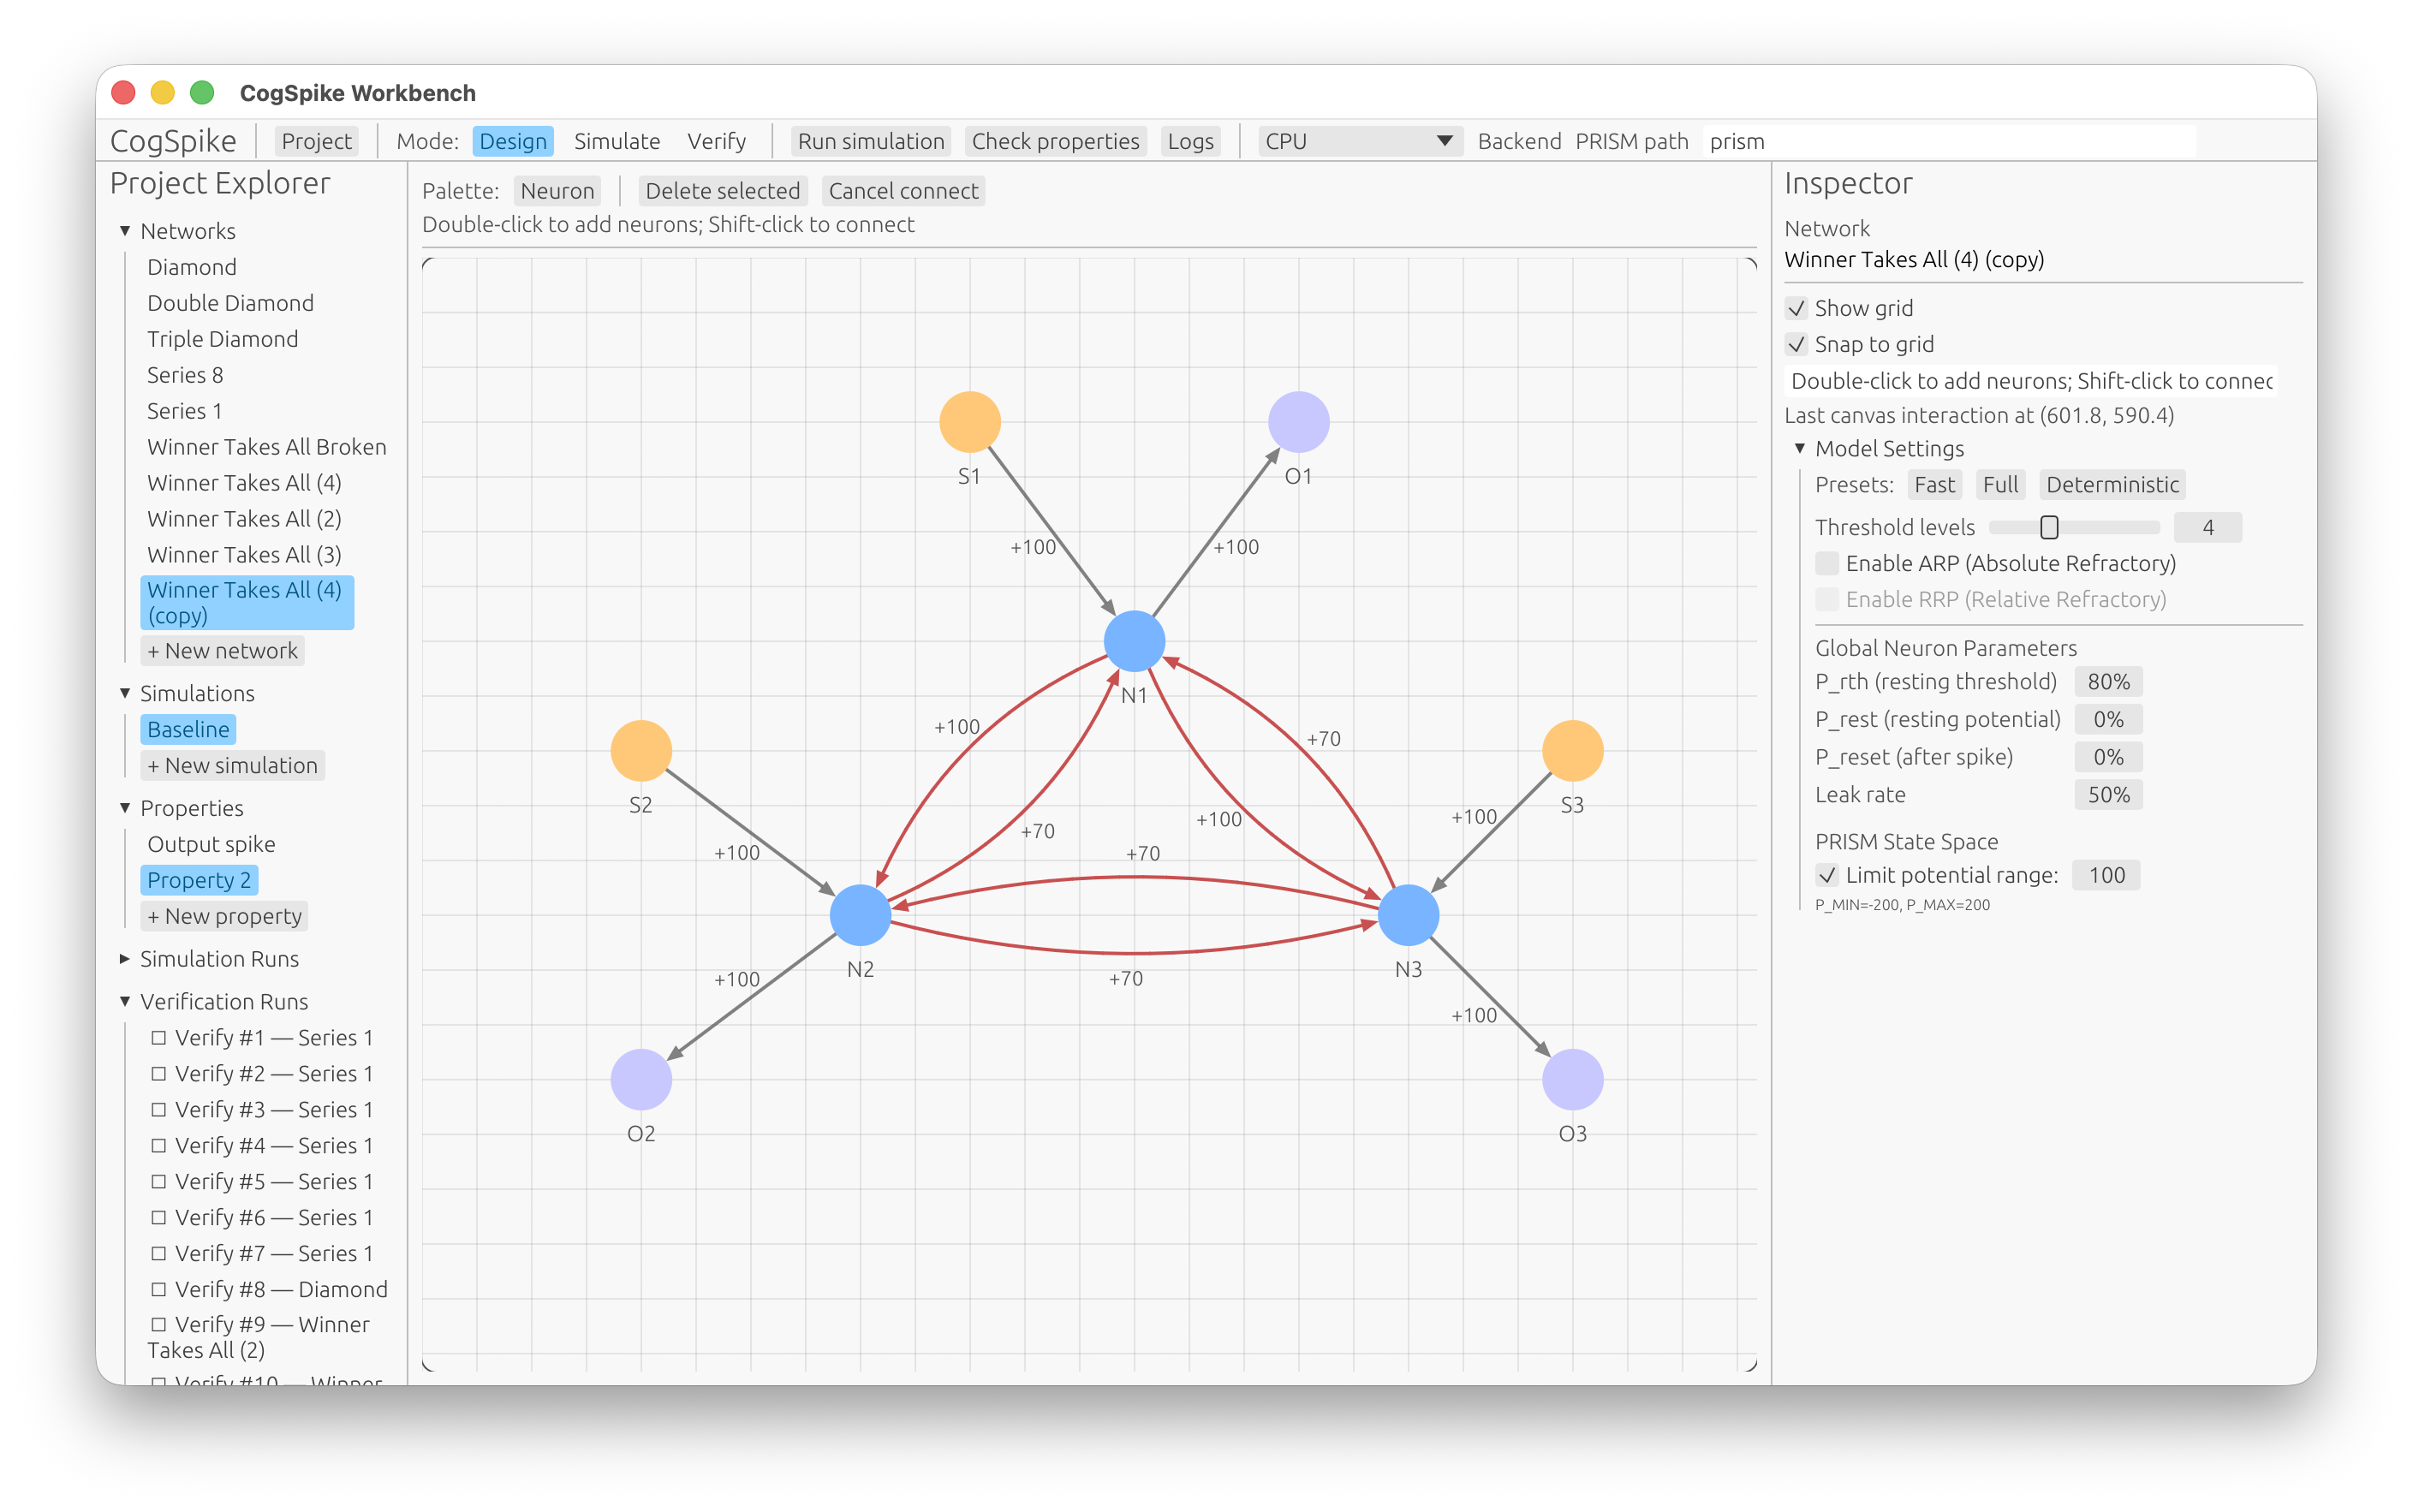
\includegraphics[width=\textwidth]{cogspike.png}
\caption{The CogSpike workbench showing the contralateral inhibition topology:
  input neurons (orange, S1--S3), competing processing neurons (blue, N1--N3)
  with mutual inhibitory connections (red edges), and output neurons (purple,
  O1--O3).}
\label{fig:cogspike}
\end{figure}

\subsection{State Space Reduction}

To quantify the impact of weight discretization on this topology, we compare the
reachable state space of the \emph{precise} PRISM model against the
\emph{weight-discretized} model ($W = 6$), both using the non-refractory
configuration ($k = 4$ threshold levels, no ARP/RRP).

The precise model yields 3,603 reachable states and 9,917 transitions, while the
$W = 6$ discretized model reduces this to just 387 states and 1,000 transitions,
that is, a $\mathbf{9.3\times}$ \emph{state} reduction and a $\mathbf{9.9\times}$
\emph{transition} reduction. This compression is especially notable given the
recurrent inhibitory connections of the network. The saving is not specific to
this topology: across seven canonical feedforward motifs the per-neuron reduction
compounds at roughly $17\times$ per neuron (for $W = 3$), growing exponentially
with network size. The full topology-by-topology measurements appear in the
extended version~\cite{cogspikeExtended}.

\subsection{Formal Verification of Winner-Takes-All Dynamics}

Table~\ref{tab:wta} reports the PCTL verification results on both models. Three
properties characterize classical Winner-Takes-All behaviour: the predetermined
winner (N1) must fire infinitely often, and both losers (N2, N3) must eventually
become permanently silent.

\begin{table}[t]
\caption{PCTL verification results on both the precise model (3,603 states, 9,917
  transitions) and the discretized $W = 6$ model (387 states, 1,000
  transitions).}
\label{tab:wta}
\centering
\setlength{\tabcolsep}{8pt}
\renewcommand{\arraystretch}{1.25}
\begin{tabular}{llll}
\hline
\textbf{PCTL Property} & \textbf{Precise} & \textbf{Disc. $W$=6} &
  \textbf{Interpretation}\\
\hline
$P_{=?}[\mathbf{G}\mathbf{F}(y_{\mathrm{N1}} = 1)]$ & 1.0 & 1.0 &
  Winner fires infinitely often\\
$P_{=?}[\mathbf{F}\mathbf{G}(y_{\mathrm{N2}} = 0)]$ & 1.0 & 1.0 &
  Loser N2 eventually silent\\
$P_{=?}[\mathbf{F}\mathbf{G}(y_{\mathrm{N3}} = 0)]$ & 1.0 & 1.0 &
  Loser N3 eventually silent\\
\hline
\end{tabular}
\end{table}

Both models verify all three WTA properties with identical probabilities: the
asymmetric weight advantage makes N1 the persistent winner, while both losers are
driven to permanent silence. The discretized model preserves these properties
exactly with only $387$ states---a $9.3\times$ reduction from $3{,}603$---demonstrating
substantial compression without loss of verification fidelity.


% ═══════════════════════════════════════════════════════════════════════════
\section{Conclusion}\label{sec:conclusion}

Formal verification of spiking neural networks must balance faithfulness to the
SNN model against the combinatorial explosion of exhaustive state-space
exploration. We presented a weight-discretized quotient abstraction that maps
continuous synaptic weights to a compact integer range while preserving threshold
feasibility and preventing spurious sustained firing, maintaining the core LIF
properties of tonic spiking, integrator behaviour, and excitability. We also
introduced CogSpike, a unified workbench that integrates probabilistic SNN
design, simulation, and PRISM-based formal verification. A case study on
contralateral inhibition demonstrated the full design--simulate--verify workflow,
formally proving Winner-Takes-All dynamics in a 9-neuron network. The $W = 6$
discretized model preserves all verified properties with identical probabilities
while reducing the state space from 3,603 to 387 states---a $9.3\times$ reduction.

Future work will pursue automated $W$ selection from fan-in analysis and a
PCTL-guided parameter-learning facility, in which property violations trigger
targeted corrective updates until the key specifications are satisfied with
probability close to~1.


\begin{credits}
\subsubsection{\discintname}
The authors have no competing interests to declare that are relevant to the
content of this article.
\end{credits}


% ---- Bibliography ----
\bibliographystyle{splncs04}
\bibliography{refs}

\end{document}
